\section{Programmierung}

\subsubsection{Beweisführung}

Da ist sich bei dem von uns entwickeltem System um einen Prototyp für ein nutzbaren TDN handelt, hat eine aussagekräftige Beweisführung der Geräusch-Lokalisierungen eine hohe Priorität. Zum Vorbild genommen wurden dafür herkömmliche \glqq Blitzer\grqq, bei denen ein Beweisfoto aufgenommen wird und Metadaten über die gemessene Geschwindigkeit abgespeichert und übermittelt werden.

Das eigentliche Foto wird mithilfe eines Raspberry Pi Kameramodul aufgenommen, bearbeitet und mit einem Zeitstempel versehen abgespeichert. 

Der hierzu verwendete Programmablauf lässt sich folgendermaßen beschreiben: 

%\begin{figure}[h]
%	\begin{center}
%		\includegraphics[scale=0.1]{Sections/Programmierung/Beweisführung}
%	\end{center}
%	\caption{Beweisführung}
%	\label{fig:Beweisführung}
%\end{figure

Die Beweisführung startet, wenn ein definierter Pegel überschritten wird und die Quelle des Geräusches ermittelt wurde. Da die Kamera nur einen Betrachtungswinkel von \ang{67} aufweist, wird nun überprüft, ob sich die Quelle innerhalb des Betrachtungswinkels, also innerhalb des Kamerabildes befindet\footnote{https://www.raspberrypi.org/documentation/hardware/camera/}.

Ist dem der Fall, so wird ein Kamerabild aufgezeichnet und ein Zeitstempel erstellt. Um die Komplexität des Systems möglichst gering halten zu können wird die Kameraansteuerung direkt in dem Hauptprogramm mithilfe einer Wrapper-klasse realisiert. 

Diese nutzt die \glqq RaspiCam: C++ API\grqq\ von Rafael Muñoz Salinas, um die Hardware direkt in dem Programmablauf ansteuern zu können\footnote{https://www.uco.es/investiga/grupos/ava/node/40}. Dies erspart die Zusätzliche Verwendung von Unterprogrammen. Das nun aufgezeichnete Bild wird zunächst als \glqq .ppm\grqq\ abgespeichert. 

In dem nächsten Schritt wird das abgespeicherte Bild wieder geöffnet und mit der Bildverarbeitungsbibliothek \glqq OpenCv\grqq\ bearbeitet\footnote{https://opencv.org/about/}. Dieser Schritt wird durchgeführt, um die Errechneten Quellkoordinaten des Geräusches grafisch darzustellen. Hierbei wird das Bild in eine vorher definierte Anzahl von Segmenten (maximal 70) unterteilt. Die rechnerisch ermittelte Gradzahl der Quelle des Geräusches wird nun auf ein Segment im Bild bezogen. Dieses wird entsprechend farblich mit einem grünen, gut sichtbaren Rechteck markiert.

Im Anschluss wird das bearbeite Bild in einem für Windows-Betriebssysteme einfach zu lesendes Format abgespeichert. Der zu Beginn der Beweisführung aufgezeichnete Zeitstempel wird nun als Dateiname verwendet.

Die Beweisführung enthält somit: ein Foto des Fahrzeugs, ein markiertes Segment, in dem sich die Quelle des Geräusches befindet und ein Zeitstempel zu welchem Datum und Uhrzeit das Fahrzeug aufgezeichnet wurde. Wahlweise können darüber hinaus auch sämtliche, sich im Buffer befindlichen Date, die zur Lokalisierung des Geräusches verwendet wurden in Tabellenform abgespeichert werden. Da es sich hierbei aber bei einem längeren Betrieb um erhebliche Datenmengen handeln würde, die den internen Speicher des Raspberry belegen würden, wurde darauf bisher verzichtet. 

\subsection{Programmablauf}

Der Programmablauf wird in diesem Abschnitt Schritt für Schritt erklärt und anhand geeigneter Diagramme dargestellt. Zu einer genauen Übersicht des Ablaufes ist der Flowchart des Programmes (\autoref{fig:MainFlowchart}) hilfreich. Nun eine chronologische Erklärung der Programmteile.

%\begin{figure}[h]
%	\begin{center}
%		\includegraphics[scale=0.1]{Sections/Programmierung/MainFlowchart}
%	\end{center}
%	\caption{Main Flowchart}
%	\label{fig:MainFlowchart}
%\end{figure}


\subsubsection{doaV2}

Nach dem Programmaufruf wird die DOA Konfiguration, bestehend aus vorberechneten Werten, ausgelesen. Dies wird durch die doaV2 Klasse mithilfe der loadPrecalculatedValues Methode ermöglicht (s. Figure 1).

Hier wird zunächst die Konfigurationsdatei geöffnet. Nun werden für alle möglichen Mikrofonpaare alle vorberechneten Laufzeiten aller möglichen Winkel eingelesen und in das Array precalculatedCompareValues abgespeichert. Zuletzt wird der Zugriff auf die Datei gestoppt. Die DOA Klasse beinhaltet auch die Berechnung des Ursprungsortes eines Geräusches, auf die im späteren Programmverlauf weiter eingegangen wird.

%\begin{figure}[h]
%	\begin{center}
%		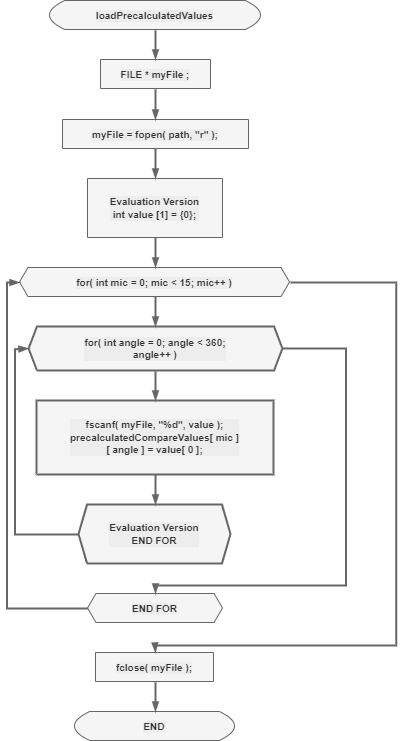
\includegraphics[scale=0.1]{Sections/Programmierung/doav2}
%	\end{center}
%	\caption{doav2}
%	\label{fig:doav2}
%\end{figure}


\subsubsection{create\_pipe}

Nach dem Laden der Laufzeiten wird mithilfe der create\_pipe Methode ein FIFO angelegt, mit dem die Echtzeitmessungen zur Datenverarbeitung weitergegeben werden.

\subsubsection{updateValues}

Diese Methode stellt sicher, dass der Daten Buffer nach jedem FIFO Zyklus neu gefüllt ist. Die Methode bestimmt zuerst das Maximum an gemessenen Werten aus einem Zyklus und schreibt sie dann mithilfe der \textit{fastAddValue} Methode im Signed UInt32 Format in den Speicher

\subsubsection{processFFT}

Eine einfache \glqq Fast Fourier Transformation\grqq, die ein Array an komplexen Gleitkommazahlen ausgibt. Mithilfe dieser Fouriertransformation ist es möglich, die Intensität der Geräusche von der zwischengespeicherten Aufnahme herauszufinden, um diese zu vergleichen.


\subsubsection{getDataForSoundDetect}

Im Programmablauf folgt diese einfache Getter-Methode, um die gepufferten Daten aus dem FIFO zur Weiterverarbeitung in ein Array zu schieben.

\subsubsection{checkForBang}

Die checkForBang Methode ist eine der wichtigsten im gesamten Programmablauf und sitzt direkt in einer Bedingung. Wenn durch diese Methode ein lautes Signal bestätigt wird, fährt das Programm in der Verarbeitung dieses Signales fort.

Wie in \autoref{fig:checkForBang} zu erkennen, wird anfangs mithilfe der calcEnergy Methode aus derselben Klasse der Unterschied zwischen den Energieniveaus von Geräuschen ausgerechnet. Dies geschieht durch die schon erwähnte FFT. Wenn nun die errechnete Differenz den Wert 600000 überschreitet, kann davon ausgegangen werden, dass ein lautes und beobachtungswertes Event stattgefunden hat, da eine sehr hohe Energiedifferenz zu vorherigen Werten gemessen wurde.

%
%\begin{figure}[h]
%	\begin{center}
%		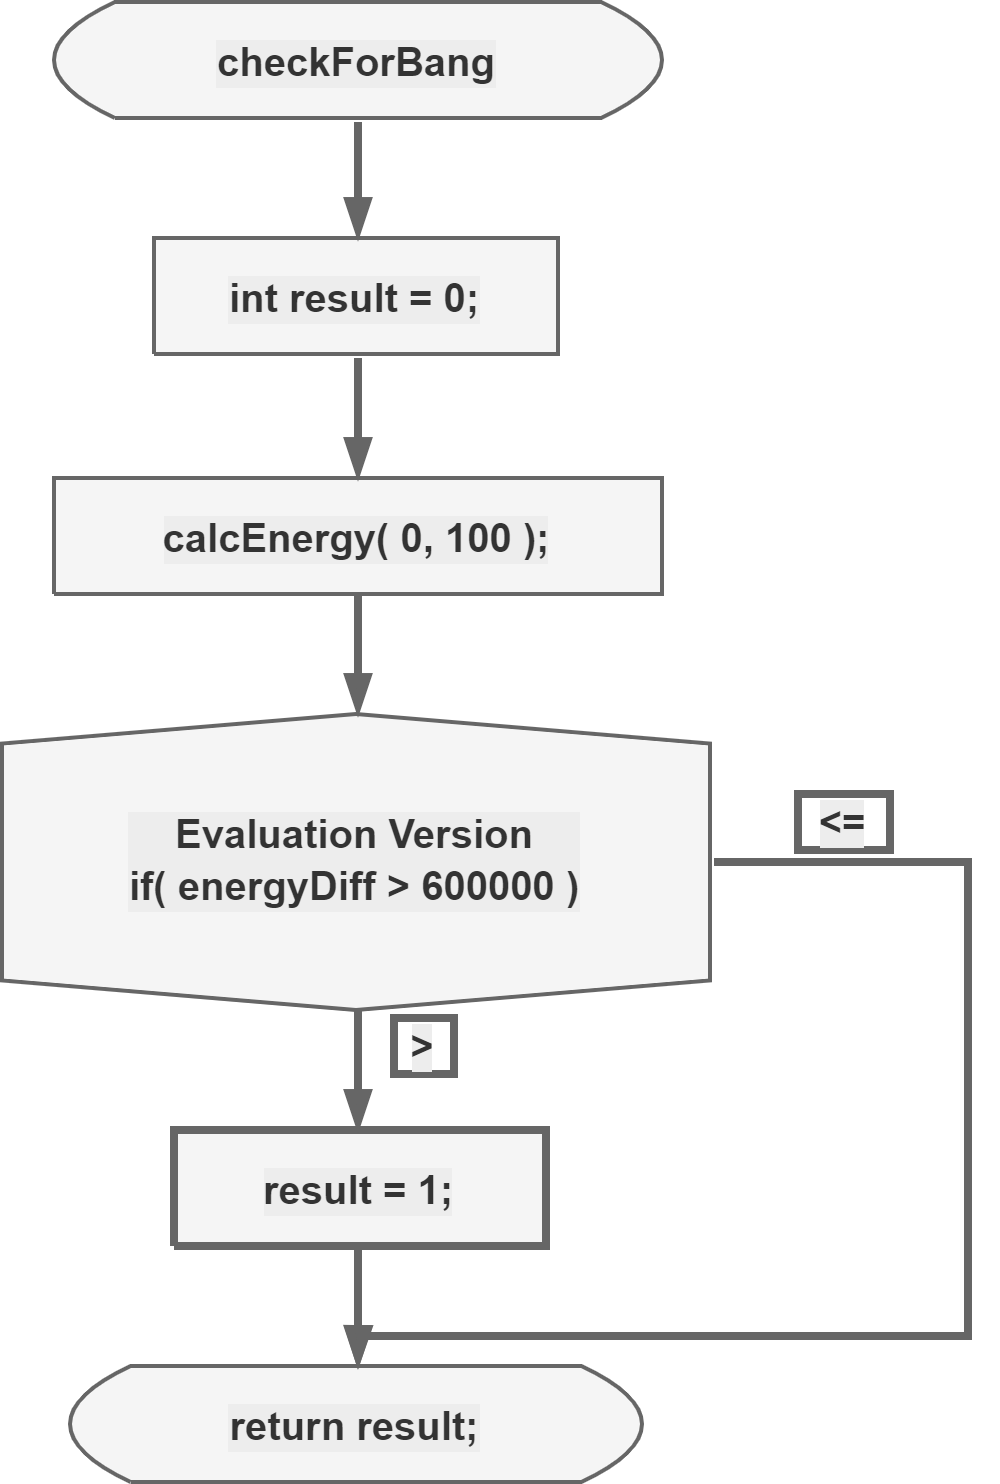
\includegraphics[scale=0.1]{Sections/Programmierung/checkForBang}
%	\end{center}
%	\caption{check for bang}
%	\label{fig:checkForBang}
%\end{figure}

\subsubsection{getAngle}

Diese Methode ist nun dafür verantwortlich, dem Geräuschevent eine eindeutige Richtung zuzuordnen, um eine Beweisführung zu ermöglichen. Sie ruft zwei weitere wichtige Methoden auf – xcorr und compareValues.

Mithilfe der vorberechneten Korrelationswerte für das Mikrofonarray kann die xcorr Methode verwendet werden, um die Korrelation zweier Signale zu finden.

Mit compareValues werden die Korrelationen verglichen und mit einer einfachen Sortierung die stärksten Übereinstimmungen gefunden, um daraus eine Richtung zu erschließen.

Mehr dazu im Abschnitt des Protokolls, dass auf die Berechnung des Winkels näher eingeht.

\subsubsection{cameraControl}

Die Klasse cameraControl benutzt nun, wenn sich der errechnete Winkel im richtigen Sichtfeld der Kamera befindet, zwei Methoden, um ein Foto zu erstellen und dies so zu bearbeiten, das der Bereich der Schallquelle sichtbar wird. Mithilfe der einfachen Schnittstelle der RaspiCam und dazugehörigen Bibliotheken wird ein Bild im RGB-Format von der Kamera angefordert und abgespeichert. Nun wird mithilfe des errechneten Ergebnisses aus getAngle und OpenCV das Bild bearbeitet, indem durch mehrere else if abfragen zum richtigen Bildsegment iteriert wird und dann dieses Segment mit einem Rechteck hervorgehoben wird.


\subsection{Ortung der Geräuschquelle}

Das Orten einer Schallquelle ist im Gegensatz zum Erfassen eines lauten Geräusches deutlich umfangreicher. Hierzu wird die Kreuzkorrelation zwischen allen Mikrofonen untereinander errechnet um diese als Hilfe zu benutzen, um das mathematische Maximum zu berechnen.

Die Kreuzkorrelation ist eine Messung, die die Bewegungen von zwei oder mehr Sätzen von Zeitreihen-Daten relativ zueinander verfolgt. Sie wird verwendet, um mehrere Zeitreihen zu vergleichen und objektiv zu bestimmen, wie gut sie miteinander übereinstimmen und insbesondere, an welchem Punkt die beste Übereinstimmung auftritt. Die Kreuzkorrelation kann auch jegliche Regelmäßigkeiten in den Daten aufdecken.

Betrachten wir als Beispiel zwei reellwertige Funktionen $ f $ und $ g $, die sich nur durch eine unbekannte Verschiebung entlang der x-Achse unterscheiden. Man kann die Kreuzkorrelation verwenden, um herauszufinden, um wie viel $ g $ entlang der x-Achse verschoben werden muss, damit es mit $ f $ identisch wird. Die Formel verschiebt im Wesentlichen die Funktion $ g $ entlang der x-Achse, wobei das Integral ihres Produkts an jeder Position berechnet wird. Wenn die Funktionen übereinstimmen, wird der Wert von ($ f \star g $) maximiert. Das liegt daran, dass Spitzen (positive Bereiche), wenn sie übereinstimmen, einen großen Beitrag zum Integral leisten. Ähnlich verhält es sich, wenn sich Talsohlen (negative Bereiche) ausrichten, leisten sie ebenfalls einen positiven Beitrag zum Integral, da das Produkt zweier negativer Zahlen positiv ist. Bei komplexwertigen Funktionen $ f $ und $ g $ stellt die Konjugierte von $ f $ sicher, dass ausgerichtete Spitzen (oder ausgerichtete Talsohlen) mit imaginären Komponenten positiv zum Integral beitragen.

Kreuzkorrelationen sind nützlich für die Bestimmung der Zeitverzögerung zwischen zwei Signalen, z. B. für die Bestimmung von Zeitverzögerungen für die Ausbreitung von akustischen Signalen über ein Mikrofonarray. Nach der Berechnung der Kreuzkorrelation zwischen den beiden Signalen zeigt das Maximum (oder Minimum, wenn die Signale negativ korreliert sind) der Kreuzkorrelationsfunktion den Zeitpunkt an, an dem die Signale am besten ausgerichtet sind; d. h., die Zeitverzögerung zwischen den beiden Signalen wird durch das Argument des Maximums die Kreuzkorrelation bestimmt. Diese mathematische Eigenschaft benutzen wir um mit
$ \tau= arg\ _{t \in \mathbb{R}}\ max\left(( f \star g)(t)\right) $ den zeitlichen Versatz zu errechnen.

In unserem Fall werden diese Maxima initial in Abhängigkeit der geometrischen Form des Mikrofonarray ausgerechnet. Dann wird in der \textit{xcorr} Methode die maximale Latenz zwischen jeder möglichen Mikrofonpaarung ausgerechnet und diese dann in der compareValues Methode miteinander verglichen. Diese Methode vergleicht nun alle gemessenen Verzögerungen mit den vorher ausgerechneten Verzögerungen, und zwar für jeden möglichen Winkel. Der Winkelbereich mit den größten Übereinstimmungen über alle Mikrofonpaarung, kann mit Sicherheit als der Bereich gekennzeichnet werden, aus dem das Geräusch kommt.

\newpage

\begin{tabularx}{\columnwidth}{|p{4cm}|X|}
	\hline
	\textbf{Abschnitt} & \textbf{Inhalt}\\
	\hline
	\textbf{Name} & Mikrofonfunktionstest\\
	\hline
	\textbf{Autor(en)} & Philipp Otto\\
	\hline
	\textbf{Priorität} & hoch\\	
	\hline	
	\textbf{Kritikalität} & hoch\\
	\hline
%	\textbf{Quelle} & \\
%	\hline
	\textbf{Verantwortlicher} & Philipp Otto\\
	\hline
	\textbf{Kurzbeschreibung} & Mit diesem Test soll die fehlerfreie Funktion der Mikrofone getestet werden\\
	\hline
	\textbf{Auslösendes Ereignis} & Eingabe Konsole: \glqq sudo ./RecordMicToRAM\grqq\\
	\hline
	\textbf{Akteure} & Mirkofonpaar, Rasberry Pi, Jumperkabel\\
	\hline
	\textbf{Vorbedingung} & Raspberry eingerichtet, Mikrofone und Raspberry mit Kabel verbunden, Raspberry eingeschaltet\\
	\hline
	\textbf{Nachbedingung} & \glqq RecordMicToRAM\grqq\ beendet,
	Prüfung der .txt-Datei ist erfolgt
	\\
	\hline
	\textbf{Ergebnis} & .txt- Datei erstellt\\
	\hline
	\textbf{Hauptszenario} & \begin{description}[font=\normalfont]
								\item[1.] Über die Konsoleneingabe wird das Programm gestartet
								\item[2.] Das Programm zeichnet ca. 8 Sekunden lang den Aikrofonausgang auf
								\item[3.] Das Programm erstellt eine .txt-Datei mit allen Messwerten
								\item[4.] Die .txt-Datei wird auf Vollständigkeit überprüft
							\end{description}\\
	\hline
	\textbf{Alternativszenario} & \begin{description}[font=\normalfont]
									\item[4.b] Die .txt-Datei enthält keine Messwerte
									\item[4.c] Kabelverbindung wird überprüft
								\end{description}\\
%	\hline
%	\textbf{Ausnahmeszenario} & \\
%	\hline
%	\textbf{Qualitäten} & \\
	\hline
\end{tabularx}
\captionof{table}{Mikrofonfunktionstest}
\label{tab:Mikrofonfunktionstest}

\begin{tabularx}{\columnwidth}{|p{4cm}|X|}
	\hline
	\textbf{Abschnitt} & \textbf{Inhalt}\\
	\hline
	\textbf{Name} & Kabelfunktionstest Nr. 1\\
	\hline
	\textbf{Autor(en)} & Philipp Otto\\
	\hline
	\textbf{Priorität} & hoch\\	
	\hline	
	\textbf{Kritikalität} & hoch\\
	\hline
	%	\textbf{Quelle} & \\
	%	\hline
	\textbf{Verantwortlicher} & Philipp Otto\\
	\hline
	\textbf{Kurzbeschreibung} & Mit diesem Test soll die fehlerfreie Funktion der Kabel getestet werden\\
	\hline
	\textbf{Auslösendes Ereignis} & Eingabe Konsole: \glqq sudo ./RecordMicToRAM\grqq\\
	\hline
	\textbf{Akteure} & gesamtes Mikrofonarray, Raspberry Pi, Kabel (lang)\\
	\hline
	\textbf{Vorbedingung} & Das Array ist vollständig mit Kabeln und Raspberry verbunden, Raspberry eingeschaltet\\
	\hline
	\textbf{Nachbedingung} & Messwerte grafisch auf Plausibilität überprüft
	\\
	\hline
	\textbf{Ergebnis} & Plot der Messwerte\\
	\hline
	\textbf{Hauptszenario} & \begin{description}[font=\normalfont]
								\item[1.] Über die Konsoleneingabe wird das Programm gestartet
								\item[2.] Das Programm zeichnet ca. 8 Sekunden lang den Mikrofonausgang auf
								\item[3.] Das Programm erstellt eine .txt-Datei mit allen Messwerten
								\item[4.] Die .txt-Datei wird mit python-script in korrektes Datenformat gebracht und in .csv konvertiert
								\item[5.] .csv wird mit Matlab eingelesen und geplottet
								\item[6.] Plot wird auf Plausibilität überprüft
							\end{description}\\
	\hline
	\textbf{Alternativszenario} & \begin{description}[font=\normalfont]
									\item[4.b] Die .txt-Datei enthält keine Messwerte
									\item[4.c] Kabelverbindung wird überprüft
									\item[6.b] Plot weist fehlerhafte Messwerte auf
								\end{description}\\
	%\hline
	%	\textbf{Ausnahmeszenario} & \\
	%	\hline
	%	\textbf{Qualitäten} & \\
	\hline
\end{tabularx}
\captionof{table}{ Kabelfunktionstest Nr. 1}
\label{tab: Kabelfunktionstest Nr. 1}


\begin{tabularx}{\columnwidth}{|p{4cm}|X|}
	\hline
	\textbf{Abschnitt} & \textbf{Inhalt}\\
	\hline
	\textbf{Name} & Kabelfunktionstest Nr. 2\\
	\hline
	\textbf{Autor(en)} & Philipp Otto\\
	\hline
	\textbf{Priorität} & hoch\\	
	\hline	
	\textbf{Kritikalität} & hoch\\
	\hline
	%	\textbf{Quelle} & \\
	%	\hline
	\textbf{Verantwortlicher} & Philipp Otto\\
	\hline
	\textbf{Kurzbeschreibung} &Mit diesem Test soll die fehlerfreie Funktion der Kabel bei halbiertem SPI-Takt getestet werden\\
	\hline
	\textbf{Auslösendes Ereignis} & Eingabe Konsole: \glqq sudo ./RecordMicToRAM64\grqq\\
	\hline
	\textbf{Akteure} & gesamtes Mikrofonarray, Raspberry Pi, Kabel (lang)\\
	\hline
	\textbf{Vorbedingung} & Das Array ist vollständig mit Kabeln und Raspberry verbunden, Raspberry eingeschaltet\\
	\hline
	\textbf{Nachbedingung} & Messwerte grafisch auf Plausibilität überprüft
	\\
	\hline
	\textbf{Ergebnis} & Plot der Messwerte\\
	\hline
	\textbf{Hauptszenario} & \begin{description}[font=\normalfont]
		\item[1.] Über die Konsoleneingabe wird das Programm gestartet
		\item[2.] Das Programm zeichnet ca. 8 Sekunden lang den Mikrofonausgang auf
		\item[3.] Das Programm erstellt eine .txt-Datei mit allen Messwerten
		\item[4.] Die .txt-Datei wird mit python-script in korrektes Datenformat gebracht und in .csv konvertiert
		\item[5.] .csv wird mit Matlab eingelesen und geplottet
		\item[6.] Plot wird auf Plausibilität überprüft
	\end{description}\\
	\hline
	\textbf{Alternativszenario} & \begin{description}[font=\normalfont]
		\item[4.b] Die .txt-Datei enthält keine Messwerte
		\item[4.c] Kabelverbindung wird überprüft
		\item[6.b] Plot weist fehlerhafte Messwerte auf
	\end{description}\\
	%\hline
	%	\textbf{Ausnahmeszenario} & \\
	%	\hline
	%	\textbf{Qualitäten} & \\
	\hline
\end{tabularx}
\captionof{table}{ Kabelfunktionstest Nr. 2}
\label{tab: Kabelfunktionstest Nr. 2}

\begin{tabularx}{\columnwidth}{|p{4cm}|X|}
	\hline
	\textbf{Abschnitt} & \textbf{Inhalt}\\
	\hline
	\textbf{Name} & Kabelfunktionstest Nr. 2\\
	\hline
	\textbf{Autor(en)} & Philipp Otto\\
	\hline
	\textbf{Priorität} & hoch\\	
	\hline	
	\textbf{Kritikalität} & hoch\\
	\hline
	%	\textbf{Quelle} & \\
	%	\hline
	\textbf{Verantwortlicher} & Philipp Otto\\
	\hline
	\textbf{Kurzbeschreibung} & Mit diesem Test soll die fehlerfreie Funktion der Kabel bei halbiertem SPI-Takt und kürzeren Kabeln getestet werden\\
	\hline
	\textbf{Auslösendes Ereignis} & Eingabe Konsole: \glqq sudo ./RecordMicToRAM64\grqq\\
	\hline
	\textbf{Akteure} & gesamtes Mikrofonarray, Raspberry Pi, Kabel (kurz)\\
	\hline
	\textbf{Vorbedingung} & Das Array ist vollständig mit Kabeln und Raspberry verbunden, Raspberry eingeschaltet\\
	\hline
	\textbf{Nachbedingung} & Messwerte grafisch auf Plausibilität überprüft
	\\
	\hline
	\textbf{Ergebnis} & Plot der Messwerte\\
	\hline
	\textbf{Hauptszenario} & \begin{description}[font=\normalfont]
		\item[1.] Über die Konsoleneingabe wird das Programm gestartet
		\item[2.] Das Programm zeichnet ca. 8 Sekunden lang den Mikrofonausgang auf
		\item[3.] Das Programm erstellt eine .txt-Datei mit allen Messwerten
		\item[4.] Die .txt-Datei wird mit python-script in korrektes Datenformat gebracht und in .csv konvertiert
		\item[5.] .csv wird mit Matlab eingelesen und geplottet
		\item[6.] Plot wird auf Plausibilität überprüft
	\end{description}\\
	\hline
	\textbf{Alternativszenario} & \begin{description}[font=\normalfont]
		\item[4.b] Die .txt-Datei enthält keine Messwerte
		\item[4.c] Kabelverbindung wird überprüft
		\item[6.b] Plot weist fehlerhafte Messwerte auf
	\end{description}\\
	%\hline
	%	\textbf{Ausnahmeszenario} & \\
	%	\hline
	%	\textbf{Qualitäten} & \\
	\hline
\end{tabularx}
\captionof{table}{ Kabelfunktionstest Nr. 3}
\label{tab: Kabelfunktionstest Nr. 3}

\begin{tabularx}{\columnwidth}{|p{4cm}|X|}
	\hline
	\textbf{Abschnitt} & \textbf{Inhalt}\\
	\hline
	\textbf{Name} & Algorithmus-Test (Matlab)\\
	\hline
	\textbf{Autor(en)} & Philipp Otto\\
	\hline
	\textbf{Priorität} & hoch\\	
	\hline	
	\textbf{Kritikalität} & hoch\\
	\hline
%	\textbf{Quelle} & \\
%	\hline
	\textbf{Verantwortlicher} & Philipp Otto\\
	\hline
	\textbf{Kurzbeschreibung} & Mit diesem Test soll die fehlerfreie Funktion des Lokalisierungs-algorithmus getestet werden\\
	\hline
	\textbf{Auslösendes Ereignis} & \glqq sudo ./RecordMicToRAM64\grqq\\
	\hline
	\textbf{Akteure} & gesamtes Mirkofonarray, Rasberry Pi, Kabel(kurz)\\
	\hline
	\textbf{Vorbedingung} & Das System ist vollständig montiert, 
	Raspberry eingeschaltet\\
	\hline
	\textbf{Nachbedingung} & Lokalisierungsergebnisse grafisch auf Plausibilität überprüft.\\
	\hline
	\textbf{Ergebnis} & Plot der Lokalisierungsergebnisse\\
	\hline
	\textbf{Hauptszenario} & \begin{description}[font=\normalfont]
								\item[1.] Über die Konsoleneingabe wird das Programm gestartet
								\item[2.] Das Programm zeichnet ca. 8 Sekunden lang den Mikrofonausgang auf
								\item[3.] Das Programm erstellt eine .txt-Datei mit allen Messwerten
								\item[4.] Die .txt-Datei wird mit python Skript in korrektes Datenformat gebracht und in .csv konvertiert
								\item[5.] .csv wird in Matlab eingelesen
								\item[6.] Lokalisierung wird mithilfe des Skripts \glqq testDelayAndSum.m\grqq\ berechnet und geplottet
								\item[7.] Plot wird auf Plausibilität überprüft
							\end{description}\\
	\hline
	\textbf{Alternativszenario} & \begin{description}[font=\normalfont]
									\item[7.b] Lokalisierung entspricht nicht dem erwarteten Winkelbereich
									\item[6.c] Lokalisierung ist uneindeutig
									\item[8.] Messung wird in anderem Umfeld wiederholt
								\end{description}\\
	\hline
	\textbf{Ausnahmeszenario} & \\
	\hline
	\textbf{Qualitäten} & \\
	\hline
\end{tabularx}
\captionof{table}{Algorithmus-Test (Matlab)}
\label{tab:Algorithmus_Test_Matlab}

\begin{tabularx}{\columnwidth}{|p{4cm}|X|}
	\hline
	\textbf{Abschnitt} & \textbf{Inhalt}\\
	\hline
	\textbf{Name} & Gesamt-Funktionstest\\
	\hline
	\textbf{Autor(en)} & Philipp Otto\\
	\hline
	\textbf{Priorität} & hoch\\	
	\hline	
	\textbf{Kritikalität} & hoch\\
	\hline
%	\textbf{Quelle} & \\
%	\hline
	\textbf{Verantwortlicher} & Philipp Otto\\
	\hline
	\textbf{Kurzbeschreibung} & Mit diesem Test soll die fehlerfreie Funktion des gesamten Programms getestet werden\\
	\hline
	\textbf{Auslösendes Ereignis} & Eingabe Konsole: \glqq sudo ./mic\_handler\_pipe64\grqq, Start des Programms über Netbeans\\
	\hline
	\textbf{Akteure} & gesamtes Mirkofonarray, Rasberry Pi, Kabel(kurz)\\
	\hline
	\textbf{Vorbedingung} & Das System ist vollständig montiert, 
	Raspberry eingeschaltet\\
	\hline
	\textbf{Nachbedingung} & Lokalisierungsergebnisse grafisch auf Plausibilität überprüft.\\
	\hline
	\textbf{Ergebnis} & Bearbeitetes .png-Datei\\
	\hline
	\textbf{Hauptszenario} & \begin{description}[font=\normalfont]
									\item[1.] Über \glqq run\grqq\ wird das Hauptprogramm in der IDE gestartet
									\item[2.] 4 Sekunden warten
									\item[3.] Mit \glqq sudo ./mic\_handler\_pipe64\grqq\ wird die pipe geöffnet
									\item[4.] Geräuschevent wird erzeugt
									\item[5.] Event wird erkannt und auf Konsole angezeigt
									\item[6.] Wenn das Event im Bildbereich erzeugt wurde, wird ein Bild aufgezeichnet
									\item[7.] Bild wird bearbeitet und abgespeichert
									\item[8.] Bild wird auf Zweitgerät geladen
									\item[9.] Bild wird auf Plausibilität überprüft
							\end{description}\\
	\hline
	\textbf{Alternativszenario} & \begin{description}[font=\normalfont]
									\item[5.b] Event wird nicht korrekt erkannt
									\item[5.c] Pegelerkennung wird angepasst
									\item[5.d] Event wird wiederholt
									\item[6.b] Event wurde im Bildbereich erzeugt aber nicht dort lokalisiert
									\item[6.c] Event wird wiederholt
									\item[9.b] Bearbeitetes Bild entspricht nicht den Erwartungen
									\item[9.c] Lokalisierungsparameter (Buffer wird angepasst)
									\item[9.d] Event wird wiederholt
									\end{description}\\
	\hline
%	\textbf{Ausnahmeszenario} & \\
%	\hline
%	\textbf{Qualitäten} & \\
%	\hline
\end{tabularx}
\captionof{table}{Gesamt-Funktionstest}
\label{tab:Gesamt-Funktionstest}

\begin{figure}[h]
	\begin{center}
		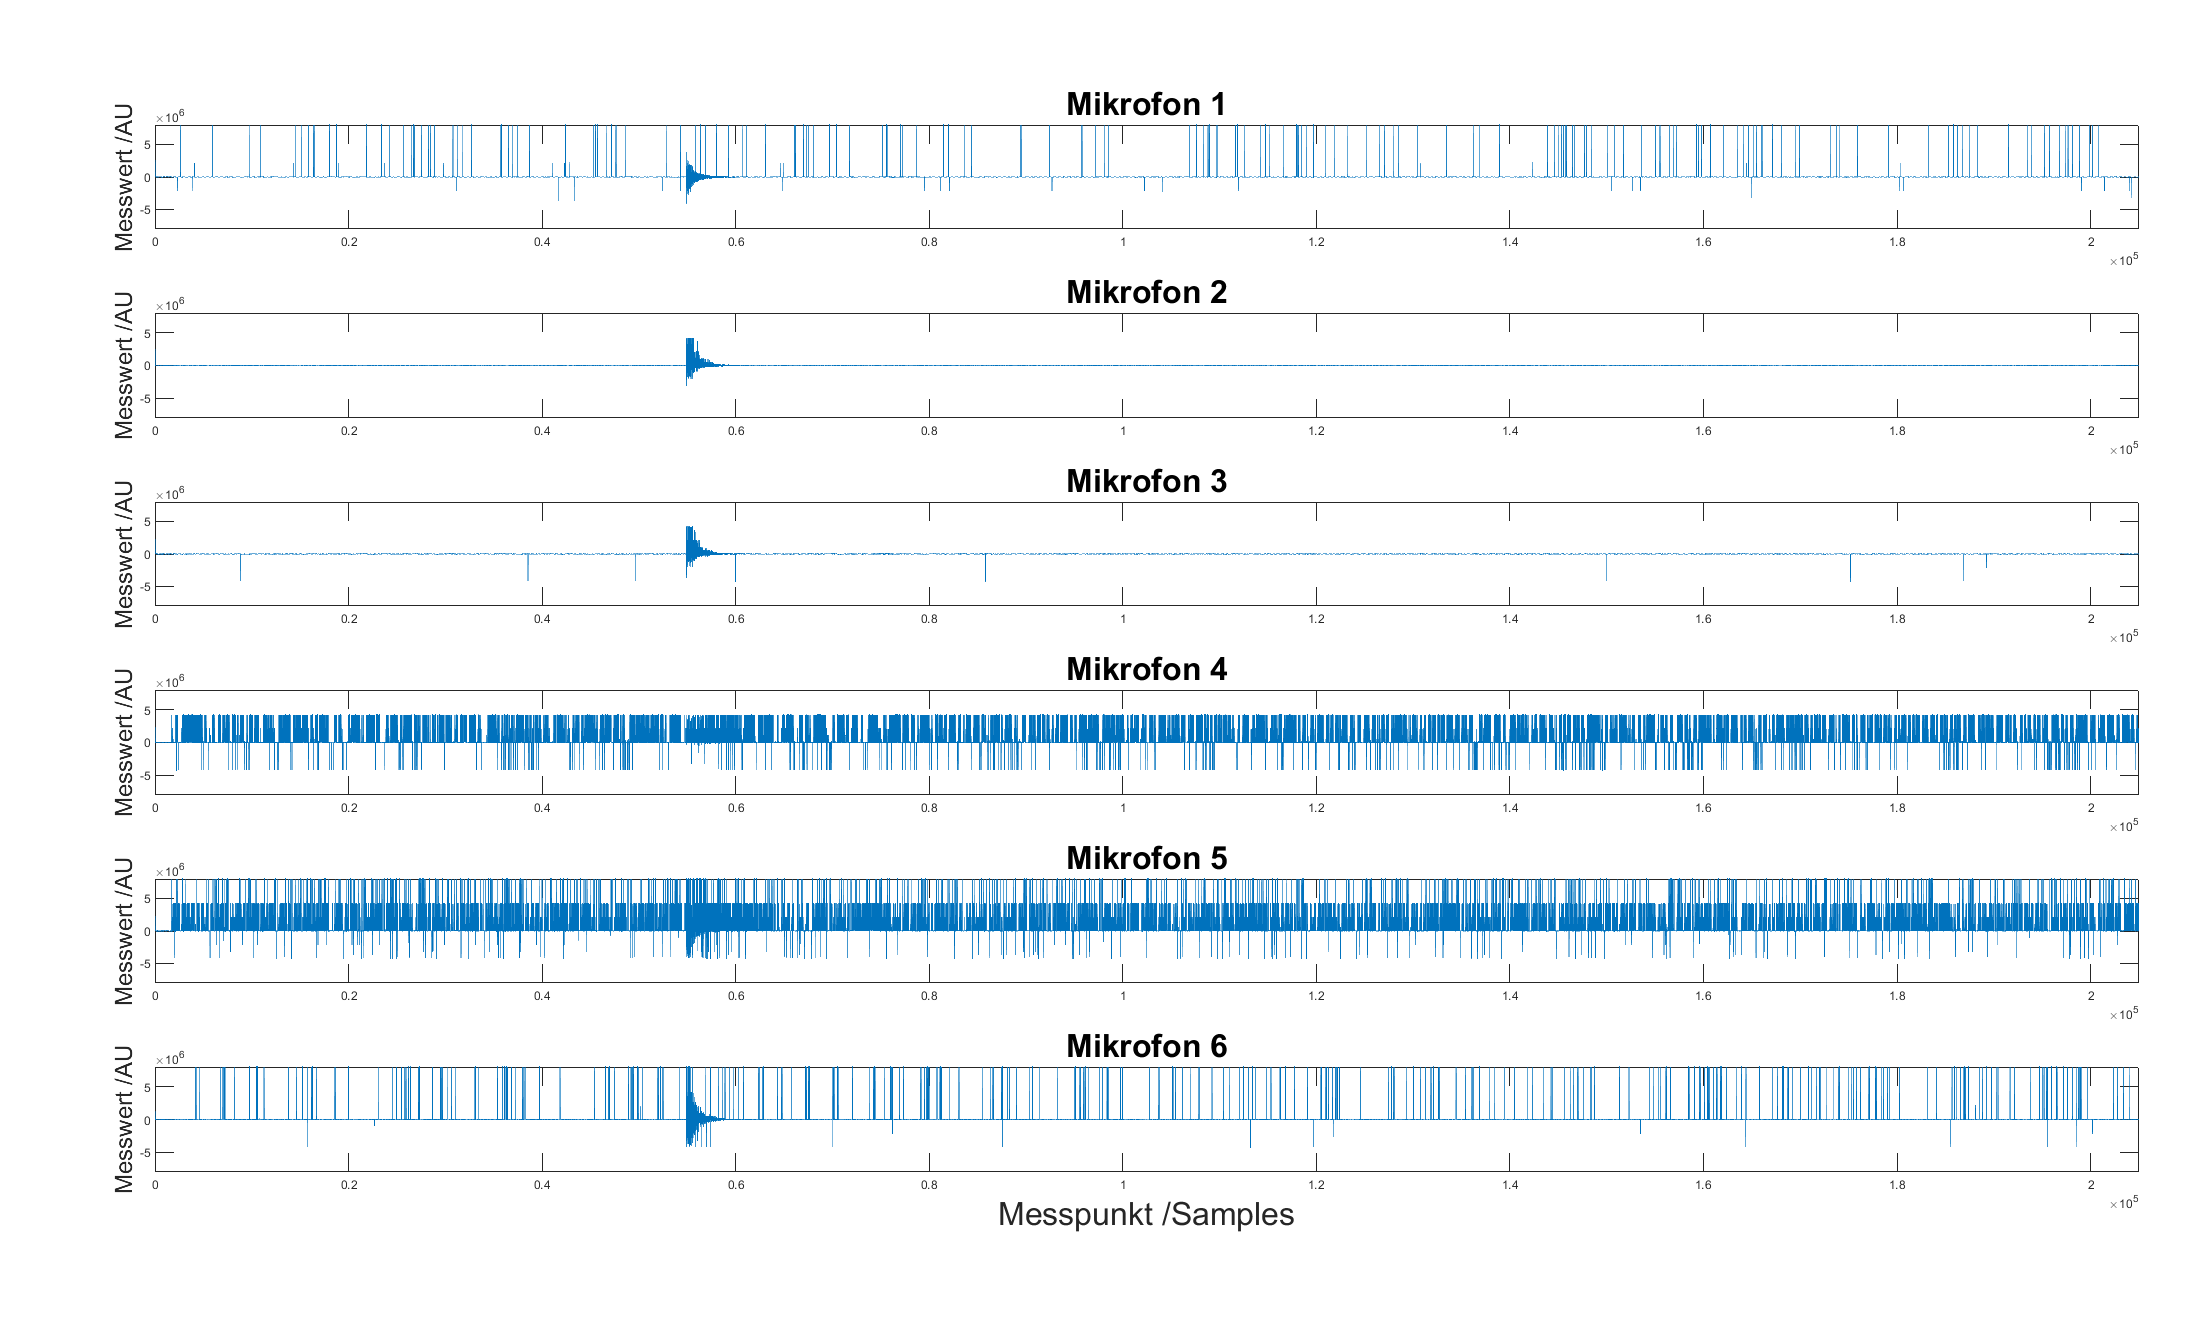
\includegraphics[width=\textwidth]{Sections/Programmierung/Test_2_d}
	\end{center}
	\caption{Test 2 d}
	\label{fig:Test_2_d}
\end{figure}

\begin{figure}[h]
	\begin{center}
		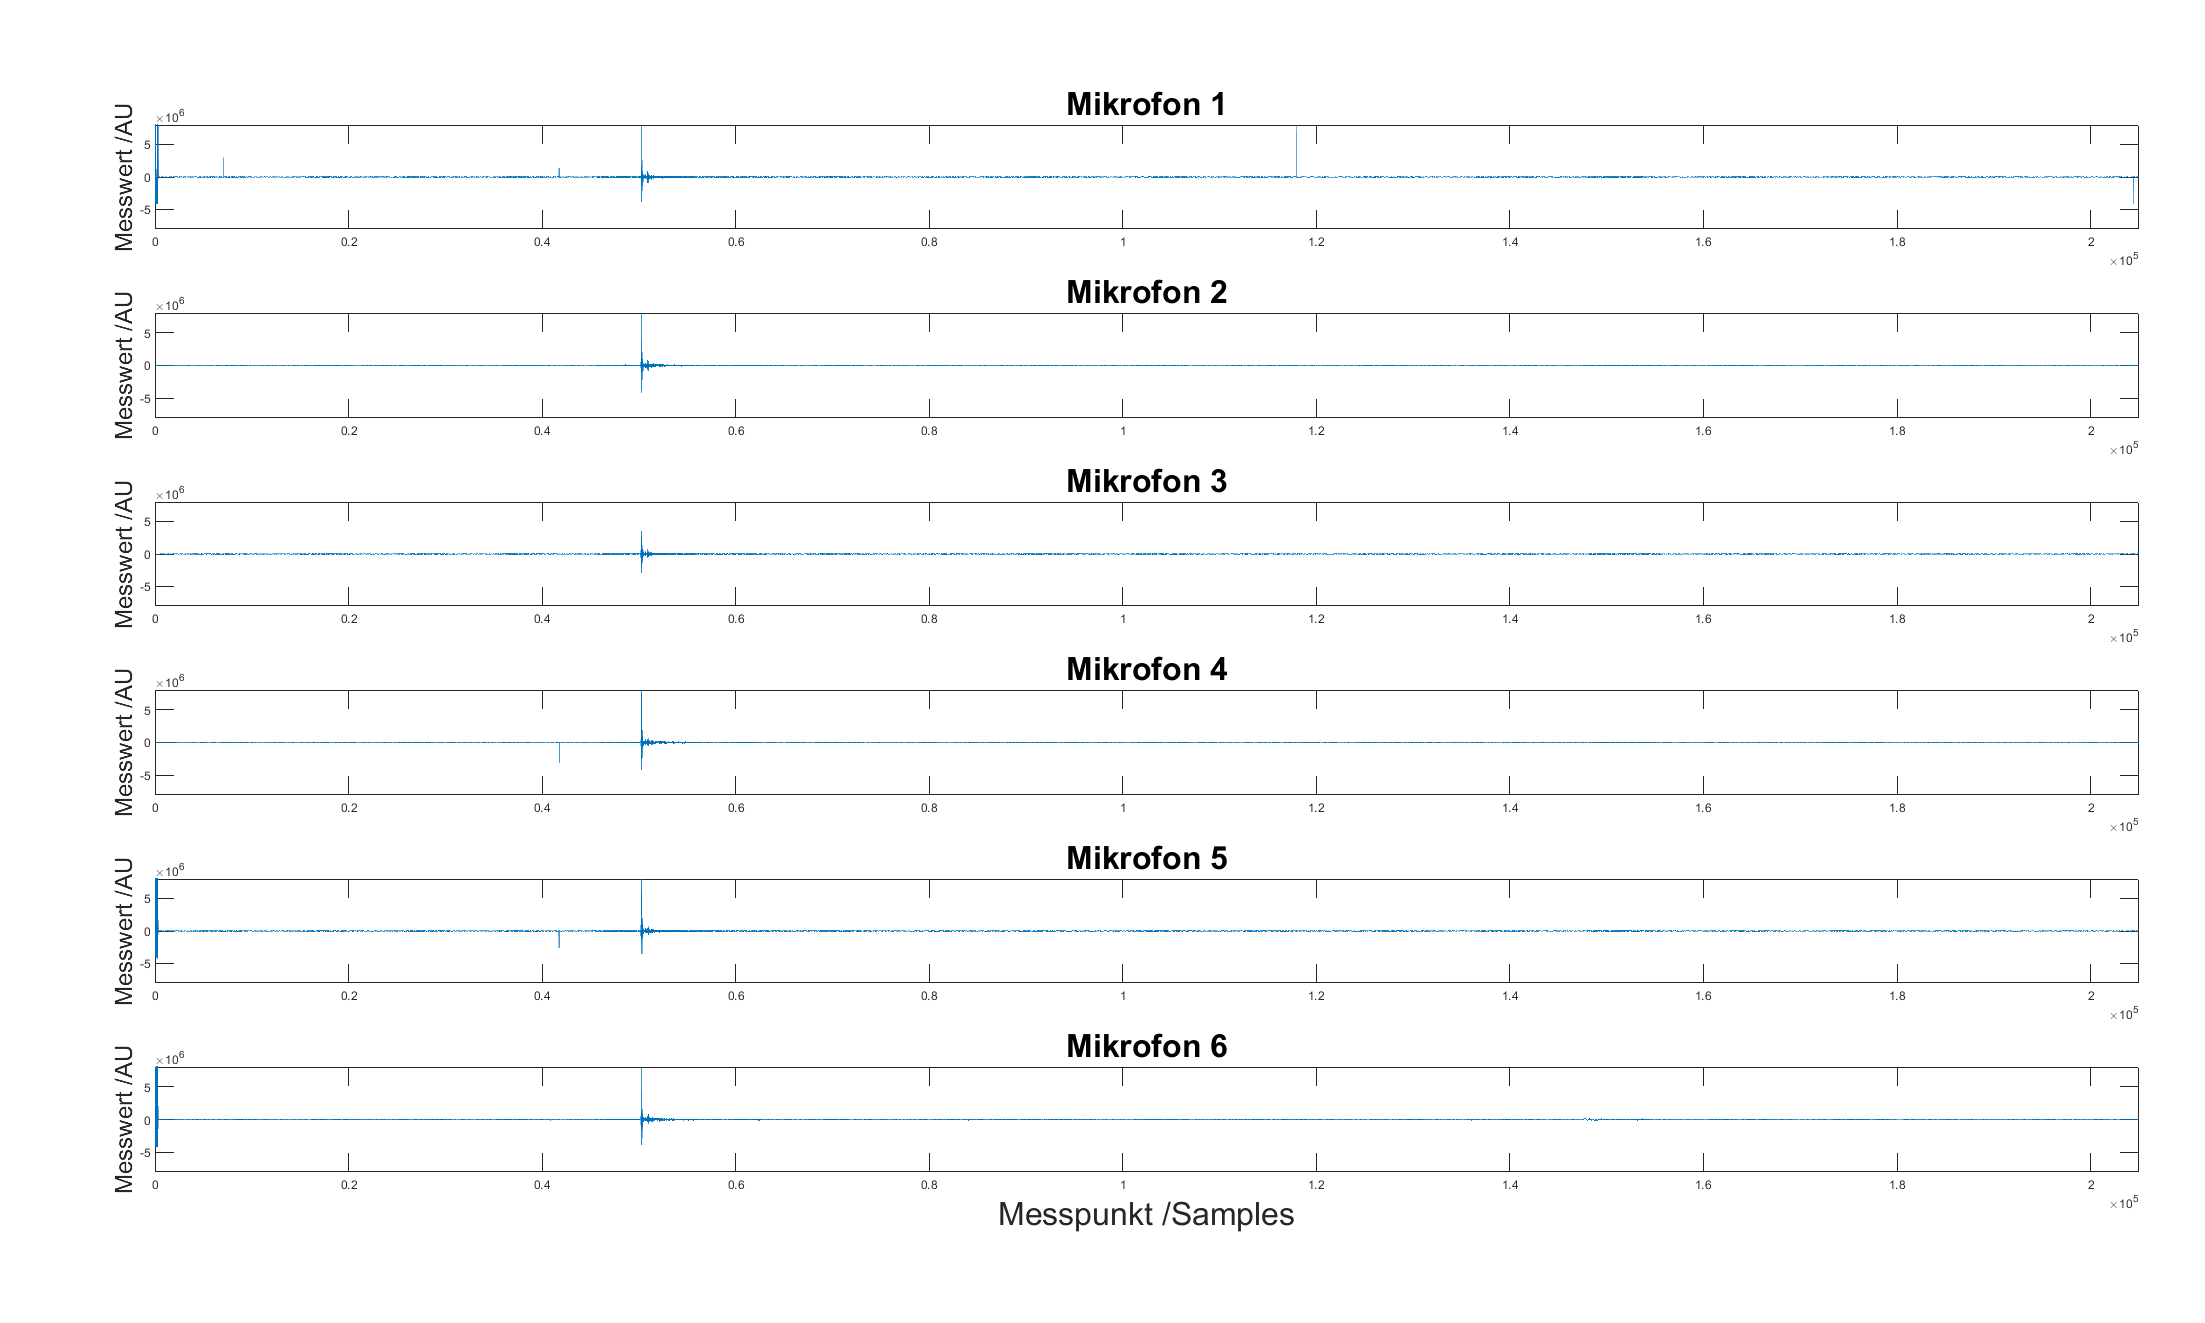
\includegraphics[width=\textwidth]{Sections/Programmierung/Test_3_d}
	\end{center}
	\caption{Test 3 d}
	\label{fig:Test_3_d}
\end{figure}

\newpage